我们已经讨论了程序的性能,还提到了高性能软件。但这些代表了什么呢?通常,我们知道高性能的程序比较快,但这并不意味着更快的程序总是有好的性能(两个程序都可能有较差的性能)。

我们也提到了高效的程序,但是效率和高性能一样吗?虽然效率与性能有关,但并不相同。效率是指有效地利用资源,而不是浪费资源,而高效的程序会充分的利用计算硬件。

一方面,高效的程序不会让可用的资源闲置。如果有需要完成的计算,而有处理器什么都不做,那么这个处理器应该正在等待执行的代码。进一步的说,处理器中有许多计算资源,高效的程序可以同时利用尽可能多的资源。而高效的程序不会浪费资源去做不必要的工作,不会执行不需要的计算,不会浪费内存去存储永远不使用的数据,在不需要的情况下,不会通过网络发送数据等。简而言之,高效的程序不会让可用的硬件闲置,也不会做不必要的工作。

另一方面,性能总是与一些指标相关。最常见的是“速度”,或程序运行的有多快。更严格地定义是\textit{吞吐量},即程序在给定时间内执行的计算量,或者说是计算特定结果所需的时间。然而,这并不是性能的唯一定义。

\subsubsubsection{1.3.1\hspace{0.2cm}性能——吞吐量}

考虑四个使用不同实现来计算相同结果的程序。下面是四个程序的运行时间(单位是相对的。实际数字并不重要,因为我们感兴趣的是相对性能):

%\hspace*{\fill} \\ %插入空行
\begin{center}
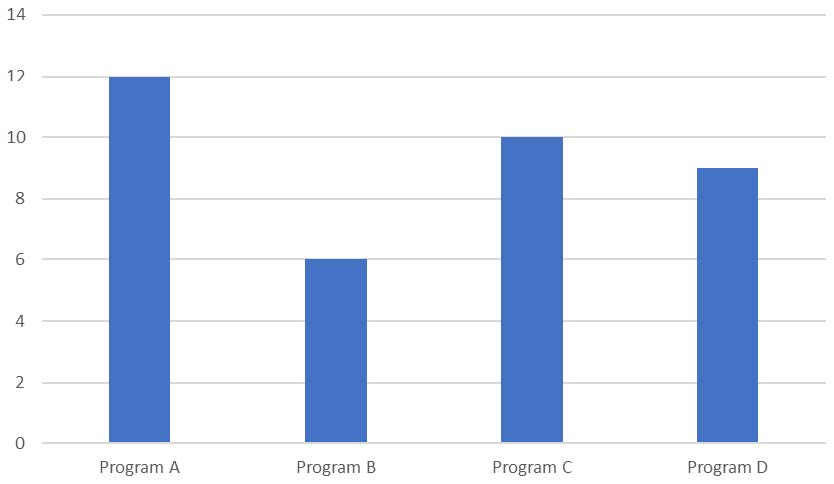
\includegraphics[width=0.8\textwidth]{content/1/chapter1/images/5.jpg}\\
图1.5 - 同一算法,四种不同实现的运行时间(相对单位)
\end{center}

显然,程序B的性能最高,比其他三个程序完成得早,计算同样结果所需的时间是最慢程序的一半。通常,这将是我们选择最佳实现所需的依据。

问题的背景很重要,我们忽略了这个程序是否是在电池供电的设备上运行的(比如手机),而且功耗指标也很重要。

\subsubsubsection{1.3.2\hspace{0.2cm}性能——功耗}

以下是四个程序在计算过程中所消耗的功率:

%\hspace*{\fill} \\ %插入空行
\begin{center}
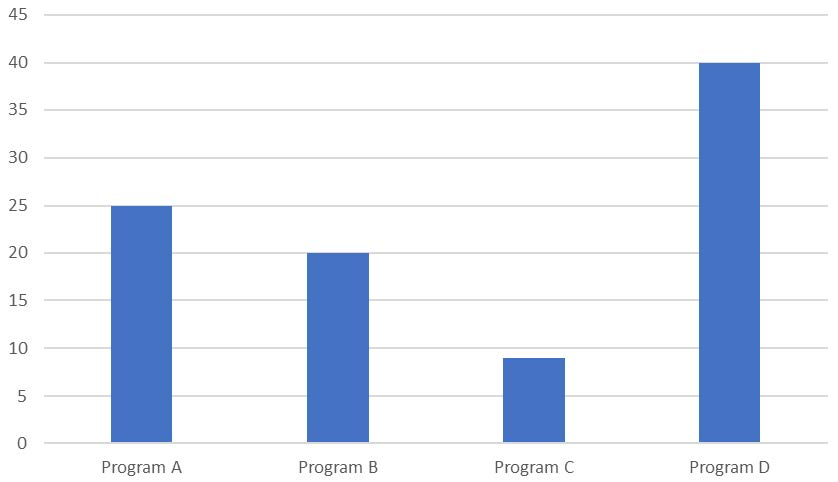
\includegraphics[width=0.8\textwidth]{content/1/chapter1/images/6.jpg}\\
图1.6 - 同一算法,四种不同实现的功耗(相对单位)
\end{center}

虽然需要更长的时间才能得到结果,但是程序C总体上使用的功率更少。那么,哪个程序的性能最好呢?

同样,这是一个不了解完整背景的陷阱问题。程序不仅在移动设备上运行,而且执行实时计算,比如:用于音频处理。这应该会让结果更快地返回,对吧?不一定哦。

\subsubsubsection{1.3.3\hspace{0.2cm}性能——实时性}

实时程序必须时刻跟上它正在处理的事件,特别对于音频处理器来说,必须跟上语音输入。假设这个程序处理音频的速度比人说话的速度快十倍,对我们来说这够快了,所以不妨把注意力转向功耗。

一方面,如果程序偶尔会落后于输入,这样一些声音甚至文字就会消失。这说明实时或速度在一定程度上很重要,但必须以可知的方式进行交付。

当然,对此也有一个性能指标:尾部延迟。延迟是指数据准备好(语音记录)和处理完成之间的延迟。前面的吞吐量反映了处理声音的平均时间,如果对着手机说一个小时,那么音频处理器需要多长时间来完成所有计算?这种情况下,真正重要的是每个声音的计算都需要按时完成。

在底层上,计算速度会波动:有时计算完成得快,有时时间会长。要是平均速度可以接受,那重点就在于是罕见的长延迟上了。

尾部延迟是作为延迟的特定百分位数来计算的,例如:如果$ t $有$95^{th}$个百分位的延迟,那么95\%的所有计算花费的时间会比t少。指标本身是$95^{th}$个百分位时间$ t $与平均计算时间$ t_0 $的比率(经常表示为百分比,所以$95^{th}$个百分位的30\%延迟意味着$ t $比$ t_0 $大30\%):

%\hspace*{\fill} \\ %插入空行
\begin{center}
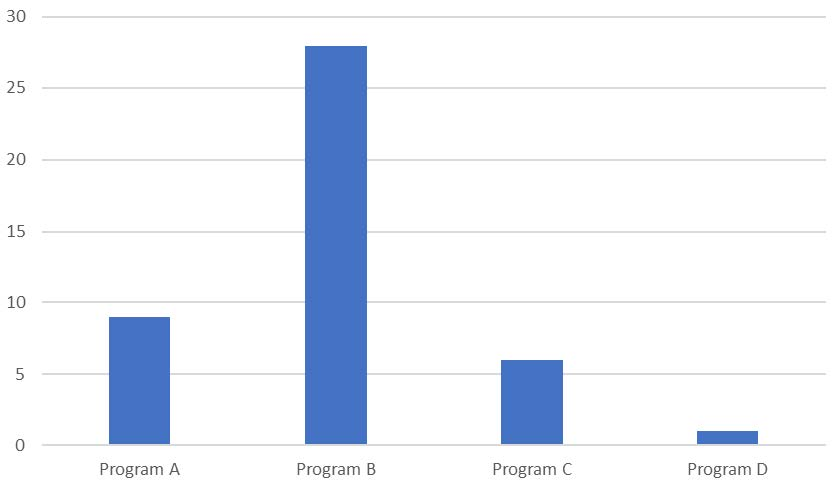
\includegraphics[width=0.9\textwidth]{content/1/chapter1/images/7.jpg}\\
图1.7 - 95\%相同算法的四种不同实现的延迟(百分比)
\end{center}

平均下来程序B的计算结果比其他任何实现都快,它也提供了最不可预测的运行时间结果。而程序D的计算像发条一样精确,每次做一个给定的计算几乎花费相同的时间。我们已经观察到,程序D的功耗是最差的。这很罕见,因为使程序更节能的技术,本质上是概率性的。大多数时候会加快计算速度,但也并不是每次都会这样。

那么,哪个程序的性能最好呢?答案肯定取决于程序,但即便如此,区别也可能并不明显。

\subsubsubsection{1.3.4\hspace{0.2cm}性能——依赖上下文}

如果这是在大型数据中心中运行的仿真软件,并且需要花费数天的时间来计算,那么吞吐量就非常重要了。对于电池供电的设备,功耗通常是最重要的。在更复杂的环境中,比如实时音频处理器,可能会是多个性能指标的组合。当然,平均运行时间也很重要,但只有当它“足够快”时才重要。如果说话者没有注意到延迟,处理的更快一点也什么意义。需要注意尾部延迟,用户的耐心会随着漏词,一点点的消耗殆尽。当延迟足够好,通话质量则会受到其他因素的限制,那再关注这个点就没什么意义了,这时可以注意下能耗。

我们现在了解了,与效率不同,性能总是根据特定的指标来定义的,这些指标取决于应用程序和具体使用场景。对于某些指标来说,当其他指标出现时,就会出现“足够好”的情况。效率反映了计算资源的利用情况,是实现良好性能的方法(可能是最常见的方法,但不是唯一的方法)。











